% SMART-R — architecture diagram set
%
% Follows the C4 model (https://c4model.com), the common standard for
% architecture diagrams that must serve technical and non-technical readers.
% Four levels, each answering one question for one audience:
%
%   1. System context   — what is this, who uses it      (everyone)
%   2. Containers       — what are the moving parts      (everyone; some detail)
%   3. Deployment       — where does it run              (engineers)
%   4. Message journey  — what happens to one message    (everyone; some detail)
%
% Naming rule: every box is Name / [Type] / one plain-English line. The name and
% description read with no background knowledge; the bracketed type is there for
% engineers and can be skipped by everyone else. Internal shorthand — repository
% names, endpoint paths, "utterance", "worker", "hub" — appears only in the
% bracketed type line, never as a box's name.
%
% Every page carries a legend, a scope line and a date, per the same standard.
%
% Build:  tectonic docs/architecture.tex
%
% Editing notes, each learned the hard way:
%   - Nodes sit at explicit coordinates, not `positioning` chains, so moving one
%     box cannot silently shift the rest.
%   - A TikZ style may NOT be named `small`: it collides with the font command
%     pgf expands internally and fails as an undefined \tikzscope@linewidth.
%   - A \\ inside a nested {\tiny ...} group breaks pgf's line splitter. Close
%     and reopen the group around the break instead.

\documentclass[11pt]{article}

\usepackage[a3paper,landscape,margin=1.1cm]{geometry}
\usepackage{tikz}
% tectonic runs XeTeX, so fontspec gives the real Unicode glyphs the labels use.
\usepackage{fontspec}
\setmainfont{Helvetica}
\setmonofont{Menlo}[Scale=0.86]
\usepackage{parskip}
\usetikzlibrary{arrows.meta, positioning, fit, backgrounds, calc}

\pagestyle{empty}

% Narrow boxes + justified text = words broken mid-syllable. Turn hyphenation
% off everywhere; ragged edges read better than "lan-guage".
\hyphenpenalty=10000
\exhyphenpenalty=10000
\tolerance=1000

%% ════════════════════════════════════════════════
%% Palette. Colour encodes one thing only: who owns
%% the box. The legend on every page says so.
%% ════════════════════════════════════════════════
\definecolor{personc}{RGB}{86,74,118}
\definecolor{studyc}{RGB}{31,95,153}
\definecolor{chatc}{RGB}{193,101,29}
\definecolor{datac}{RGB}{26,127,87}
\definecolor{extc}{RGB}{116,116,124}
\definecolor{inkc}{RGB}{31,35,40}
\definecolor{mutec}{RGB}{110,118,129}

\tikzset{
  box/.style={
    rectangle, rounded corners=3pt, draw, thick,
    text width=3.5cm, align=center, inner sep=5pt,
    font=\footnotesize, text=inkc, minimum height=1.5cm
  },
  wide/.style={text width=4.7cm},
  person/.style={box, fill=personc!14, draw=personc, rounded corners=13pt},
  study/.style={box, fill=studyc!14, draw=studyc},
  chat/.style={box, fill=chatc!14, draw=chatc},
  store/.style={box, fill=datac!14, draw=datac},
  ext/.style={box, fill=extc!12, draw=extc},
  bound/.style={rectangle, rounded corners=9pt, draw, line width=1.2pt,
                fill=none, inner sep=13pt, densely dashed},
  arr/.style={-{Stealth[length=5pt]}, semithick, draw=mutec},
  darr/.style={{Stealth[length=5pt]}-{Stealth[length=5pt]}, semithick, draw=mutec},
  lbl/.style={font=\scriptsize, text=inkc, fill=white, inner sep=2pt, align=center},
  num/.style={font=\scriptsize\bfseries, shape=circle, draw=mutec,
              fill=white, inner sep=1.2pt, minimum size=14pt, text=inkc},
  note/.style={font=\scriptsize, text=mutec, align=left},
  life/.style={draw=mutec!55, semithick, densely dashed},
}

%% ════════════════════════════════════════════════
%% Icons. Drawn in TikZ rather than imported, so the
%% document stays self-contained and the glyphs scale
%% with the page. Each uses `pic actions`, so colour
%% and line width come from the call site.
%% ════════════════════════════════════════════════
\tikzset{
  % stored information — the standard cylinder
  dbicon/.pic={
    \draw[pic actions] (-3mm,1.6mm) arc[start angle=180, end angle=360, x radius=3mm, y radius=1mm]
      -- (3mm,1.6mm) arc[start angle=0, end angle=180, x radius=3mm, y radius=1mm] -- cycle;
    \draw[pic actions, fill=none] (-3mm,1.6mm) -- (-3mm,-2.2mm)
      arc[start angle=180, end angle=360, x radius=3mm, y radius=1mm] -- (3mm,1.6mm);
    \draw[pic actions, fill=none] (-3mm,-0.4mm)
      arc[start angle=180, end angle=360, x radius=3mm, y radius=1mm];
  },
  % a running application — a rack unit
  srvicon/.pic={
    \draw[pic actions] (-3.2mm,0.6mm) rectangle (3.2mm,2.4mm);
    \draw[pic actions] (-3.2mm,-2.4mm) rectangle (3.2mm,-0.6mm);
    \fill[pic actions, draw=none] (-2.4mm,1.2mm) rectangle (-1.8mm,1.8mm);
    \fill[pic actions, draw=none] (-2.4mm,-1.8mm) rectangle (-1.8mm,-1.2mm);
  },
  % traffic director — one line in, several out
  lbicon/.pic={
    \draw[pic actions, fill=none] (-3.4mm,0) -- (-1mm,0);
    \draw[pic actions] (-1mm,-1.8mm) rectangle (0.6mm,1.8mm);
    \draw[pic actions, fill=none] (0.6mm,0) -- (1.6mm,0) -- (1.6mm,2mm) -- (3.4mm,2mm);
    \draw[pic actions, fill=none] (1.6mm,0) -- (3.4mm,0);
    \draw[pic actions, fill=none] (1.6mm,0) -- (1.6mm,-2mm) -- (3.4mm,-2mm);
  },
  % an outside supplier — a cloud
  cloudicon/.pic={
    \draw[pic actions] (-2.6mm,-1.1mm)
      arc[start angle=270, end angle=90, radius=0.85mm]
      arc[start angle=180, end angle=0, radius=1.15mm]
      arc[start angle=150, end angle=30, radius=1.3mm]
      arc[start angle=110, end angle=-20, radius=1.15mm] -- cycle;
  },
  % a person — head and shoulders, the C4 convention
  personicon/.pic={
    \draw[pic actions] (0,1.5mm) circle (1.1mm);
    \draw[pic actions] (-2.1mm,-2.6mm) -- (-2.1mm,-1.3mm)
      .. controls (-2.1mm,0.5mm) and (2.1mm,0.5mm) .. (2.1mm,-1.3mm)
      -- (2.1mm,-2.6mm) -- cycle;
  },
  % the participant's handset
  phoneicon/.pic={
    \draw[pic actions, rounded corners=0.5mm] (-1.7mm,-2.6mm) rectangle (1.7mm,2.6mm);
    \draw[pic actions, fill=none] (-0.6mm,2mm) -- (0.6mm,2mm);
    \fill[pic actions, draw=none] (0,-2mm) circle (0.35mm);
  },
}

% Place an icon straddling a box's top-left corner, masked so it sits cleanly
% on the border. Usage: \ico{nodename}{dbicon}{colour}
\newcommand{\ico}[3]{%
  \pic[draw=#3, fill=#3!22, semithick] at ($(#1.north west)+(0.34,0.2)$) {#2};}

% Name / [type] / description — the C4 element convention.
\newcommand{\el}[3]{\textbf{#1}\\[1pt]{\tiny\color{mutec}[#2]}\\[2pt]{\scriptsize #3}}
\newcommand{\es}[2]{\textbf{#1}\\[1pt]{\tiny\color{mutec}[#2]}}

\newcommand{\pagehead}[3]{%
  {\Large\bfseries #1}\\[3pt]
  {\small\color{mutec} #2}\\[3pt]
  {\scriptsize\color{mutec} #3}\\[12pt]
}

\newcommand{\swatch}[2]{%
  \tikz\node[fill=#1!#2, draw=#1, rounded corners=2pt,
             minimum width=0.42cm, minimum height=0.26cm]{};}
\newcommand{\swatchp}{%
  \tikz\node[fill=personc!14, draw=personc, rounded corners=7pt,
             minimum width=0.42cm, minimum height=0.26cm]{};}

% Legend repeated on every page, so the notation is never in question.
\newcommand{\legend}{%
  
\begin{tikzpicture}[baseline]
    \node[draw=mutec!40, rounded corners=5pt, fill=mutec!5, inner sep=8pt,
          align=left, font=\scriptsize, text=inkc] {
      \textbf{How to read this page}\qquad
      \tikz[baseline=-2pt]\pic[draw=personc, fill=personc!22, semithick]{personicon};\;a person\quad
      \tikz[baseline=-2pt]\pic[draw=mutec, fill=mutec!22, semithick]{srvicon};\;a running application\quad
      \tikz[baseline=-2pt]\pic[draw=datac, fill=datac!22, semithick]{dbicon};\;stored information\quad
      \tikz[baseline=-2pt]\pic[draw=mutec, fill=mutec!22, semithick]{lbicon};\;traffic director\quad
      \tikz[baseline=-2pt]\pic[draw=extc, fill=extc!22, semithick]{cloudicon};\;outside supplier\\[4pt]
      \hspace*{1pt}\swatch{studyc}{14}\;Study \& Messaging Service\quad
      \swatch{chatc}{14}\;Chatbot Service\quad
      \tikz[baseline=-2pt]\draw[arr] (0,0) -- (0.55,0);\;an arrow points at whatever is being asked to do something\quad
      {\tiny[in brackets]}\;the technology — for engineers; skip it if it means nothing to you
    };
  \end{tikzpicture}}

\begin{document}

%% ════════════════════════════════════════════════
%% 1 — SYSTEM CONTEXT  (C4 level 1)
%% The whole system as a single box. No technology.
%% This is the page to hand to someone who has never
%% seen the system before.
%% ════════════════════════════════════════════════
\null\vfill
\begin{center}
\pagehead{1 — System context}{%
  What the system is, who uses it, and what it relies on. No technical knowledge needed.}{%
  SMART-R text-messaging study \textbullet\ August 2026 \textbullet\
  Scope: the whole system as one box. What is inside it is on page 2.}

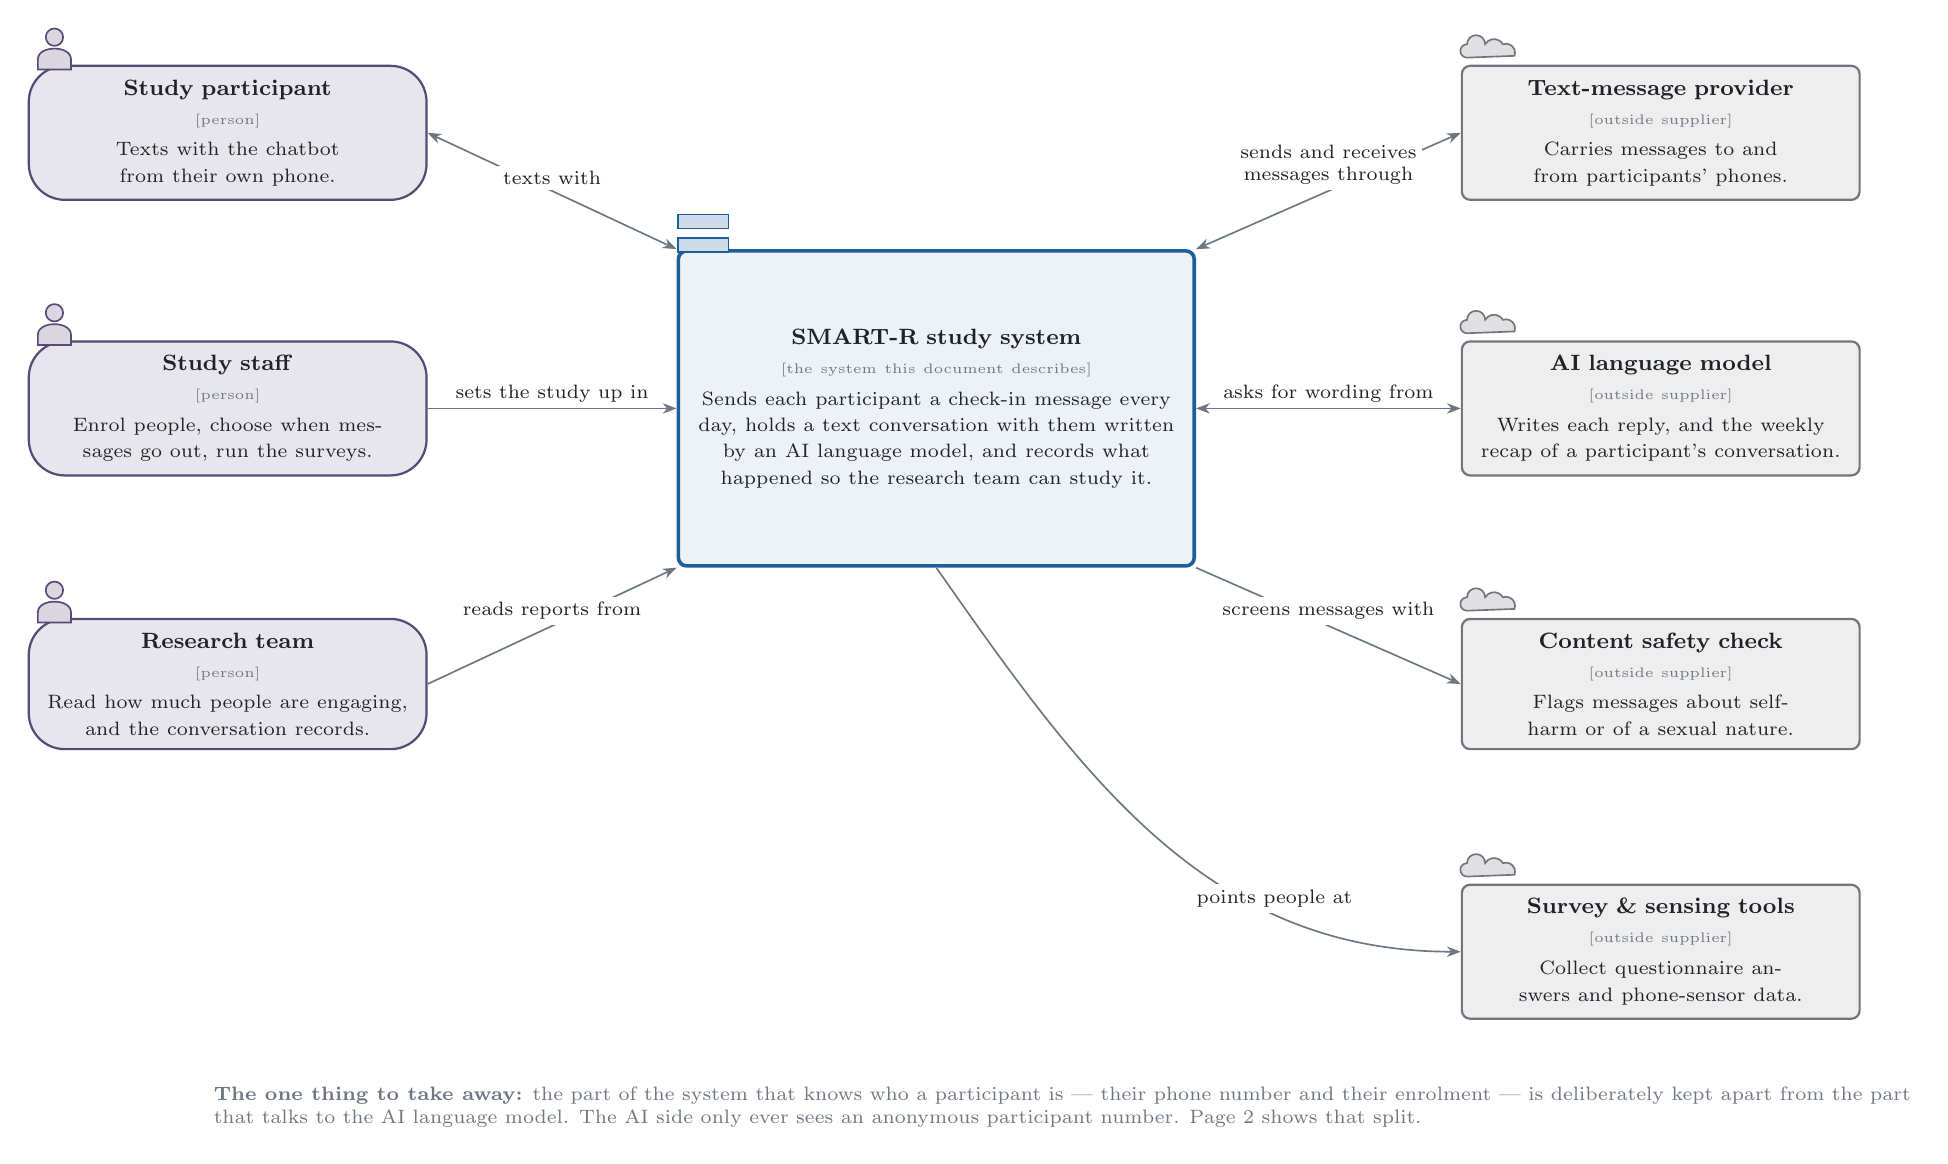
\begin{tikzpicture}

  \node[person, wide] (participant) at (0,0)
    {\el{Study participant}{person}{Texts with the chatbot from their own phone.}};
  \node[person, wide] (staff) at (0,-3.5)
    {\el{Study staff}{person}{Enrol people, choose when messages go out, run the surveys.}};
  \node[person, wide] (research) at (0,-7.0)
    {\el{Research team}{person}{Read how much people are engaging, and the conversation records.}};

  \node[box, fill=studyc!8, draw=studyc, line width=1.3pt,
        text width=6.2cm, minimum height=4cm] (system) at (9.0,-3.5)
    {\el{SMART-R study system}{the system this document describes}{%
      Sends each participant a check-in message every day, holds a text conversation
      with them written by an AI language model, and records what happened so the
      research team can study it.}};

  \node[ext, wide] (sms) at (18.2,0)
    {\el{Text-message provider}{outside supplier}{Carries messages to and from participants' phones.}};
  \node[ext, wide] (ai) at (18.2,-3.5)
    {\el{AI language model}{outside supplier}{Writes each reply, and the weekly recap of a participant's conversation.}};
  \node[ext, wide] (safety) at (18.2,-7.0)
    {\el{Content safety check}{outside supplier}{Flags messages about self-harm or of a sexual nature.}};
  \node[ext, wide] (survey) at (18.2,-10.4)
    {\el{Survey \& sensing tools}{outside supplier}{Collect questionnaire answers and phone-sensor data.}};

  \ico{participant}{personicon}{personc}
  \ico{staff}{personicon}{personc}
  \ico{research}{personicon}{personc}
  \ico{sms}{cloudicon}{extc}
  \ico{ai}{cloudicon}{extc}
  \ico{safety}{cloudicon}{extc}
  \ico{survey}{cloudicon}{extc}
  \ico{system}{srvicon}{studyc}

  \draw[darr] (participant.east) -- node[lbl, above]{texts with} (system.north west);
  \draw[arr] (staff.east) -- node[lbl, above]{sets the study up in} (system.west);
  \draw[arr] (research.east) -- node[lbl, above]{reads reports from} (system.south west);

  \draw[darr] (system.north east) -- node[lbl, above]{sends and receives\\messages through} (sms.west);
  \draw[darr] (system.east) -- node[lbl, above]{asks for wording from} (ai.west);
  \draw[arr] (system.south east) -- node[lbl, above]{screens messages with} (safety.west);
  \draw[arr] (system.south) to[out=-55, in=180] node[lbl, pos=0.72, above]{points people at} (survey.west);

  \node[note, anchor=north west] at (-0.3,-12.0)
    {\textbf{The one thing to take away:} the part of the system that knows who a participant is —
     their phone number and their enrolment — is deliberately kept apart from the part\\
     that talks to the AI language model. The AI side only ever sees an anonymous participant
     number. Page 2 shows that split.};

\end{tikzpicture}

\vspace{12pt}
\legend
\end{center}
\vfill

\clearpage

%% ════════════════════════════════════════════════
%% 2 — CONTAINERS  (C4 level 2)
%% The system opened into its two services and their
%% two stores.
%% ════════════════════════════════════════════════
\null\vfill
\begin{center}
\pagehead{2 — The parts inside}{%
  The system is two separate services with two separate stores of information.
  They say only two things to each other.}{%
  SMART-R text-messaging study \textbullet\ August 2026 \textbullet\
  Scope: applications and stored information. Servers and networks are on page 3.}

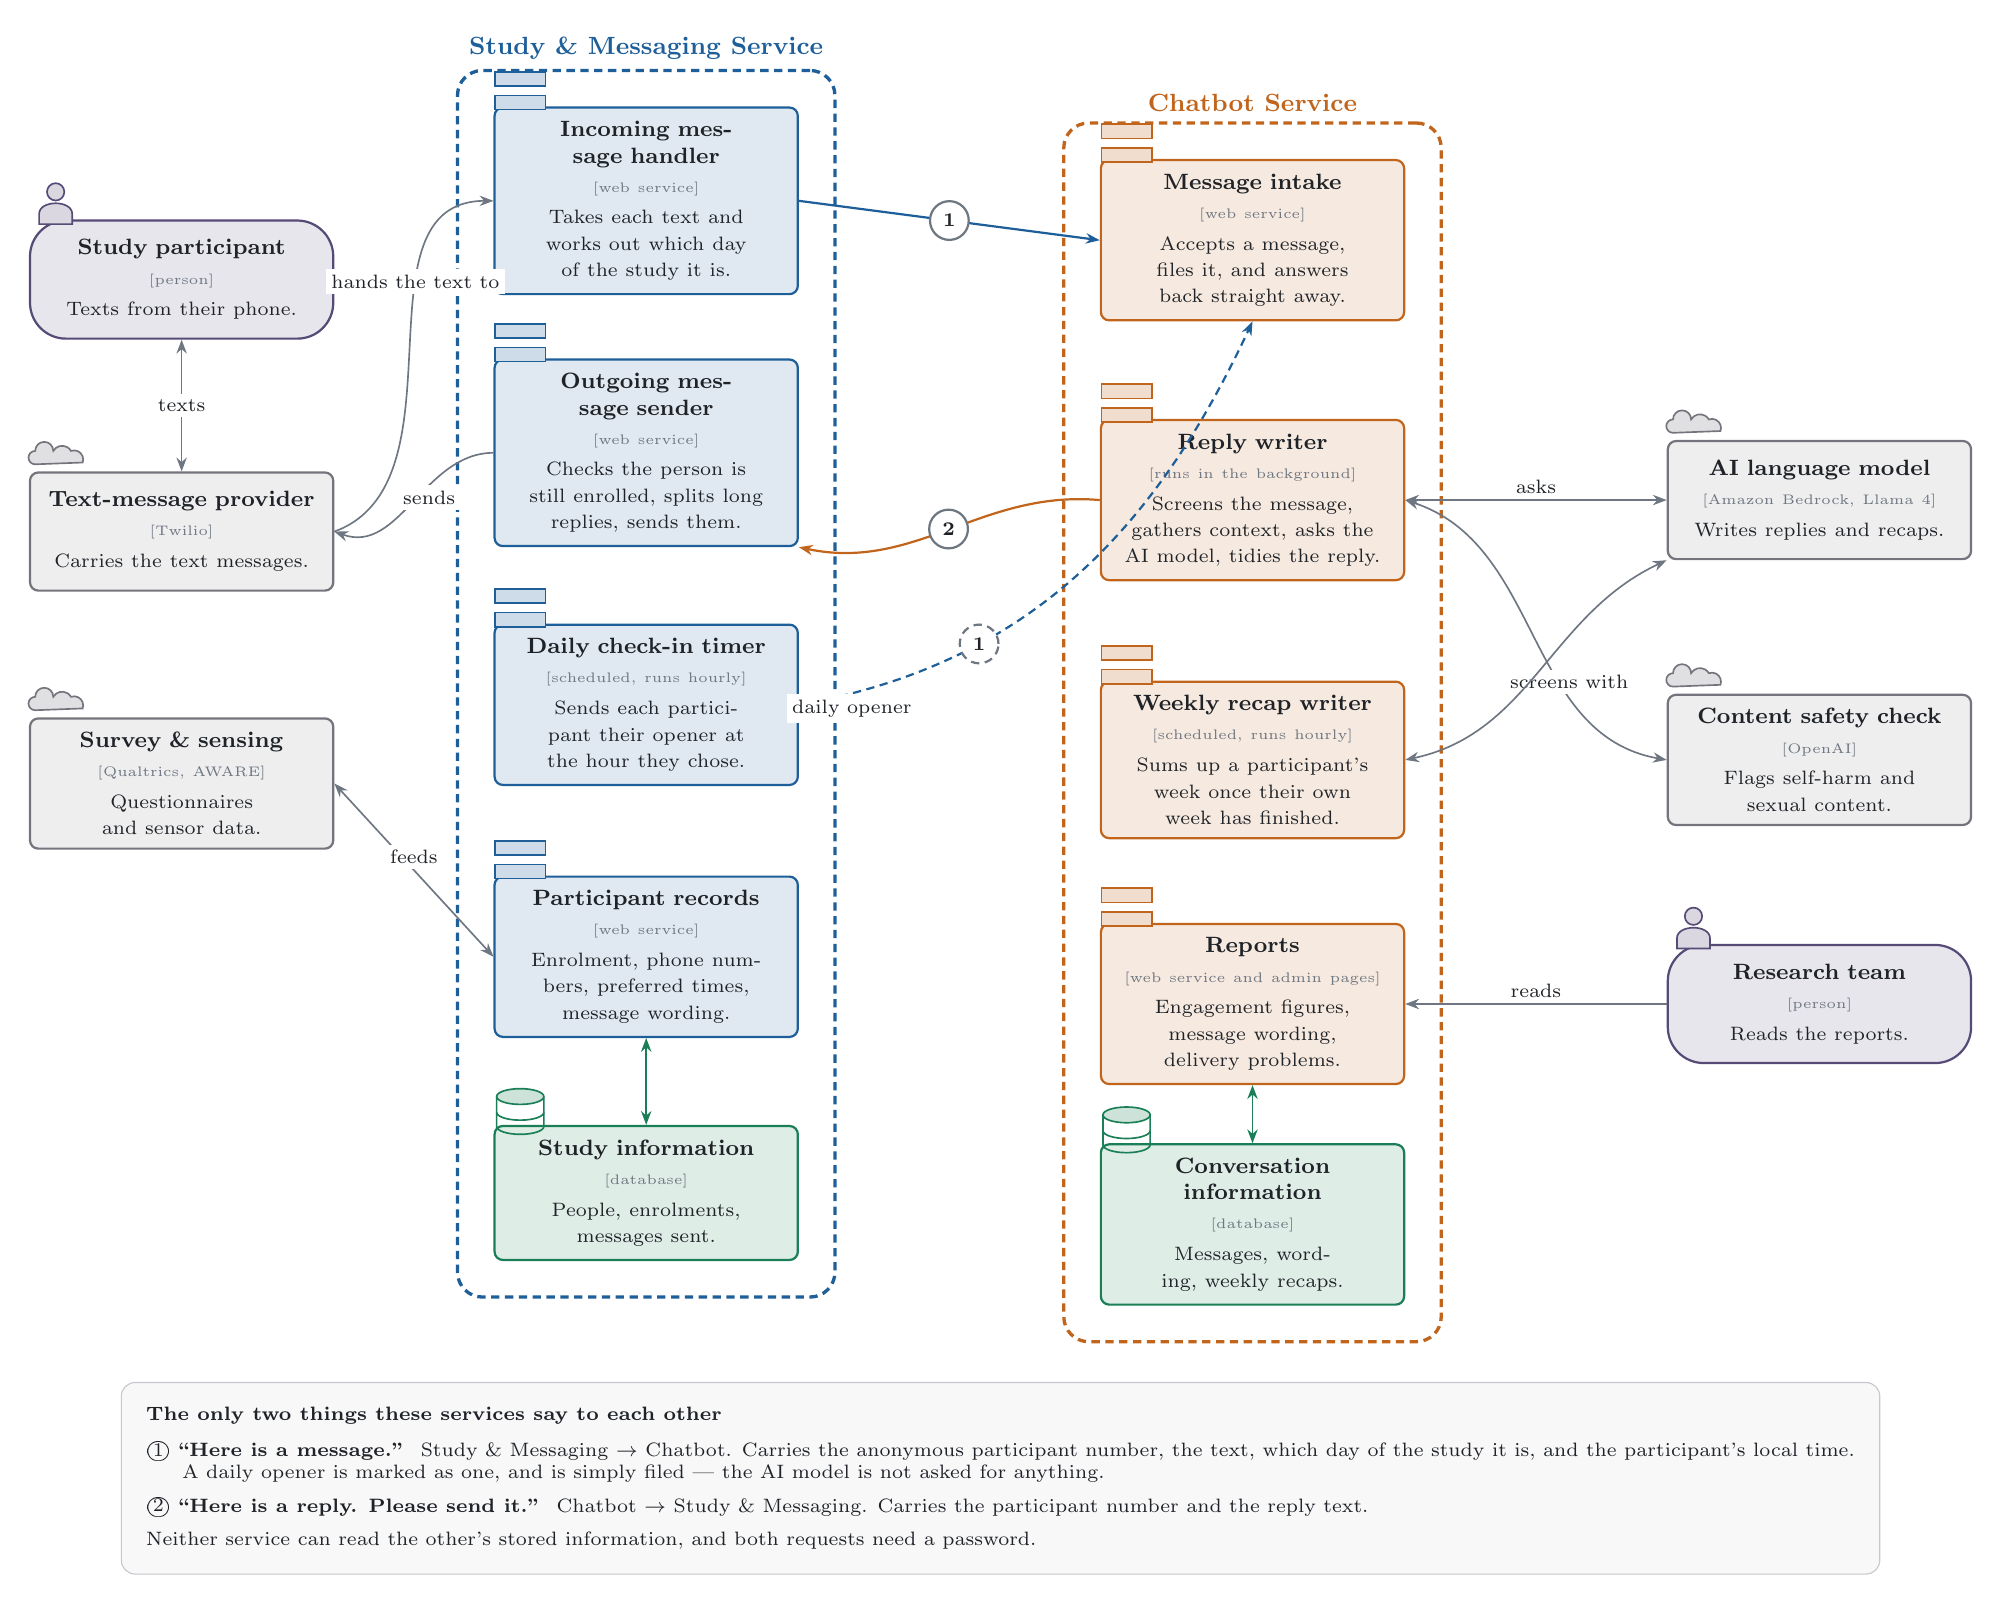
\begin{tikzpicture}

  \node[person] (participant) at (0,-1.0)
    {\el{Study participant}{person}{Texts from their phone.}};
  \node[ext] (sms) at (0,-4.2)
    {\el{Text-message provider}{Twilio}{Carries the text messages.}};
  \node[ext] (survey) at (0,-7.4)
    {\el{Survey \& sensing}{Qualtrics, AWARE}{Questionnaires and sensor data.}};

  \node[study] (inbox) at (5.9,0)
    {\el{Incoming message handler}{web service}{Takes each text and works out which day of the study it is.}};
  \node[study] (outbox) at (5.9,-3.2)
    {\el{Outgoing message sender}{web service}{Checks the person is still enrolled, splits long replies, sends them.}};
  \node[study] (timer) at (5.9,-6.4)
    {\el{Daily check-in timer}{scheduled, runs hourly}{Sends each participant their opener at the hour they chose.}};
  \node[study] (records) at (5.9,-9.6)
    {\el{Participant records}{web service}{Enrolment, phone numbers, preferred times, message wording.}};
  \node[store] (studydb) at (5.9,-12.6)
    {\el{Study information}{database}{People, enrolments, messages sent.}};

  \begin{scope}[on background layer]
    \node[bound, draw=studyc, fit=(inbox)(outbox)(timer)(records)(studydb),
          label={[text=studyc, font=\small\bfseries]above:Study \& Messaging Service}] (studybox) {};
  \end{scope}

  \node[chat] (receive) at (13.6,-0.5)
    {\el{Message intake}{web service}{Accepts a message, files it, and answers back straight away.}};
  \node[chat] (gen) at (13.6,-3.8)
    {\el{Reply writer}{runs in the background}{Screens the message, gathers context, asks the AI model, tidies the reply.}};
  \node[chat] (recap) at (13.6,-7.1)
    {\el{Weekly recap writer}{scheduled, runs hourly}{Sums up a participant's week once their own week has finished.}};
  \node[chat] (report) at (13.6,-10.2)
    {\el{Reports}{web service and admin pages}{Engagement figures, message wording, delivery problems.}};
  \node[store] (chatdb) at (13.6,-13.0)
    {\el{Conversation information}{database}{Messages, wording, weekly recaps.}};

  \begin{scope}[on background layer]
    \node[bound, draw=chatc, fit=(receive)(gen)(recap)(report)(chatdb),
          label={[text=chatc, font=\small\bfseries]above:Chatbot Service}] (chatbox) {};
  \end{scope}

  \node[ext] (ai) at (20.8,-3.8)
    {\el{AI language model}{Amazon Bedrock, Llama 4}{Writes replies and recaps.}};
  \node[ext] (safety) at (20.8,-7.1)
    {\el{Content safety check}{OpenAI}{Flags self-harm and sexual content.}};
  \node[person] (research) at (20.8,-10.2)
    {\el{Research team}{person}{Reads the reports.}};

  \ico{participant}{personicon}{personc}
  \ico{research}{personicon}{personc}
  \ico{sms}{cloudicon}{extc}
  \ico{survey}{cloudicon}{extc}
  \ico{ai}{cloudicon}{extc}
  \ico{safety}{cloudicon}{extc}
  \ico{inbox}{srvicon}{studyc}
  \ico{outbox}{srvicon}{studyc}
  \ico{timer}{srvicon}{studyc}
  \ico{records}{srvicon}{studyc}
  \ico{studydb}{dbicon}{datac}
  \ico{receive}{srvicon}{chatc}
  \ico{gen}{srvicon}{chatc}
  \ico{recap}{srvicon}{chatc}
  \ico{report}{srvicon}{chatc}
  \ico{chatdb}{dbicon}{datac}

  \draw[darr] (participant) -- node[lbl]{texts} (sms);
  \draw[arr] (sms.east) to[out=20, in=180] node[lbl, pos=0.62, above]{hands the text to} (inbox.west);
  \draw[arr] (outbox.west) to[out=180, in=-20] node[lbl, pos=0.38, below]{sends} (sms.east);
  \draw[darr] (survey.east) -- node[lbl, above]{feeds} (records.west);

  \draw[arr, draw=studyc, thick] (inbox.east) -- node[num, pos=0.5]{1} (receive.west);
  \draw[arr, draw=studyc, thick, densely dashed] (timer.east) to[out=10, in=245]
    node[num, pos=0.3]{1} node[lbl, pos=0.08, below]{daily opener} (receive.south);
  \draw[arr, draw=chatc, thick] (gen.west) to[out=175, in=-12]
    node[num, pos=0.5]{2} (outbox.south east);

  \draw[darr] (gen.east) -- node[lbl, above]{asks} (ai.west);
  \draw[darr] (gen.east) to[out=-18, in=170] node[lbl, pos=0.68, above]{screens with} (safety.west);
  \draw[darr] (recap.east) to[out=12, in=205] (ai.south west);
  \draw[arr] (research.west) -- node[lbl, above]{reads} (report.east);

  \draw[darr, draw=datac] (records) -- (studydb);
  \draw[darr, draw=datac] (report) -- (chatdb);

  \node[draw=mutec!40, rounded corners=5pt, fill=mutec!5, inner sep=9pt,
        align=left, font=\scriptsize, text=inkc, anchor=north] at (10.4,-15.0) {
    \textbf{The only two things these services say to each other}\\[5pt]
    \textcircled{1}\;\textbf{``Here is a message.''}\; Study \& Messaging $\rightarrow$ Chatbot.
    Carries the anonymous participant number, the text, which day of the study it is,
    and the participant's local time.\\
    \hspace{1.3em} A daily opener is marked as one, and is simply filed — the AI model is not asked for anything.\\[4pt]
    \textcircled{2}\;\textbf{``Here is a reply. Please send it.''}\; Chatbot $\rightarrow$ Study \& Messaging.
    Carries the participant number and the reply text.\\[4pt]
    Neither service can read the other's stored information, and both requests need a password.
  };

\end{tikzpicture}

\vspace{10pt}
\legend
\end{center}
\vfill

\clearpage

%% ════════════════════════════════════════════════
%% 3 — DEPLOYMENT
%% Written for engineers, and labelled as such.
%% Boundaries are built inside-out so every fit()
%% has its targets already defined.
%% ════════════════════════════════════════════════
\null\vfill
\begin{center}
\pagehead{3 — Where it runs}{%
  Both services run in a single Amazon Web Services account. Each keeps its own store of
  information, and neither store can be reached from the internet.}{%
  SMART-R text-messaging study \textbullet\ August 2026 \textbullet\
  Scope: servers, networks and hosting. This page is written for engineers.}

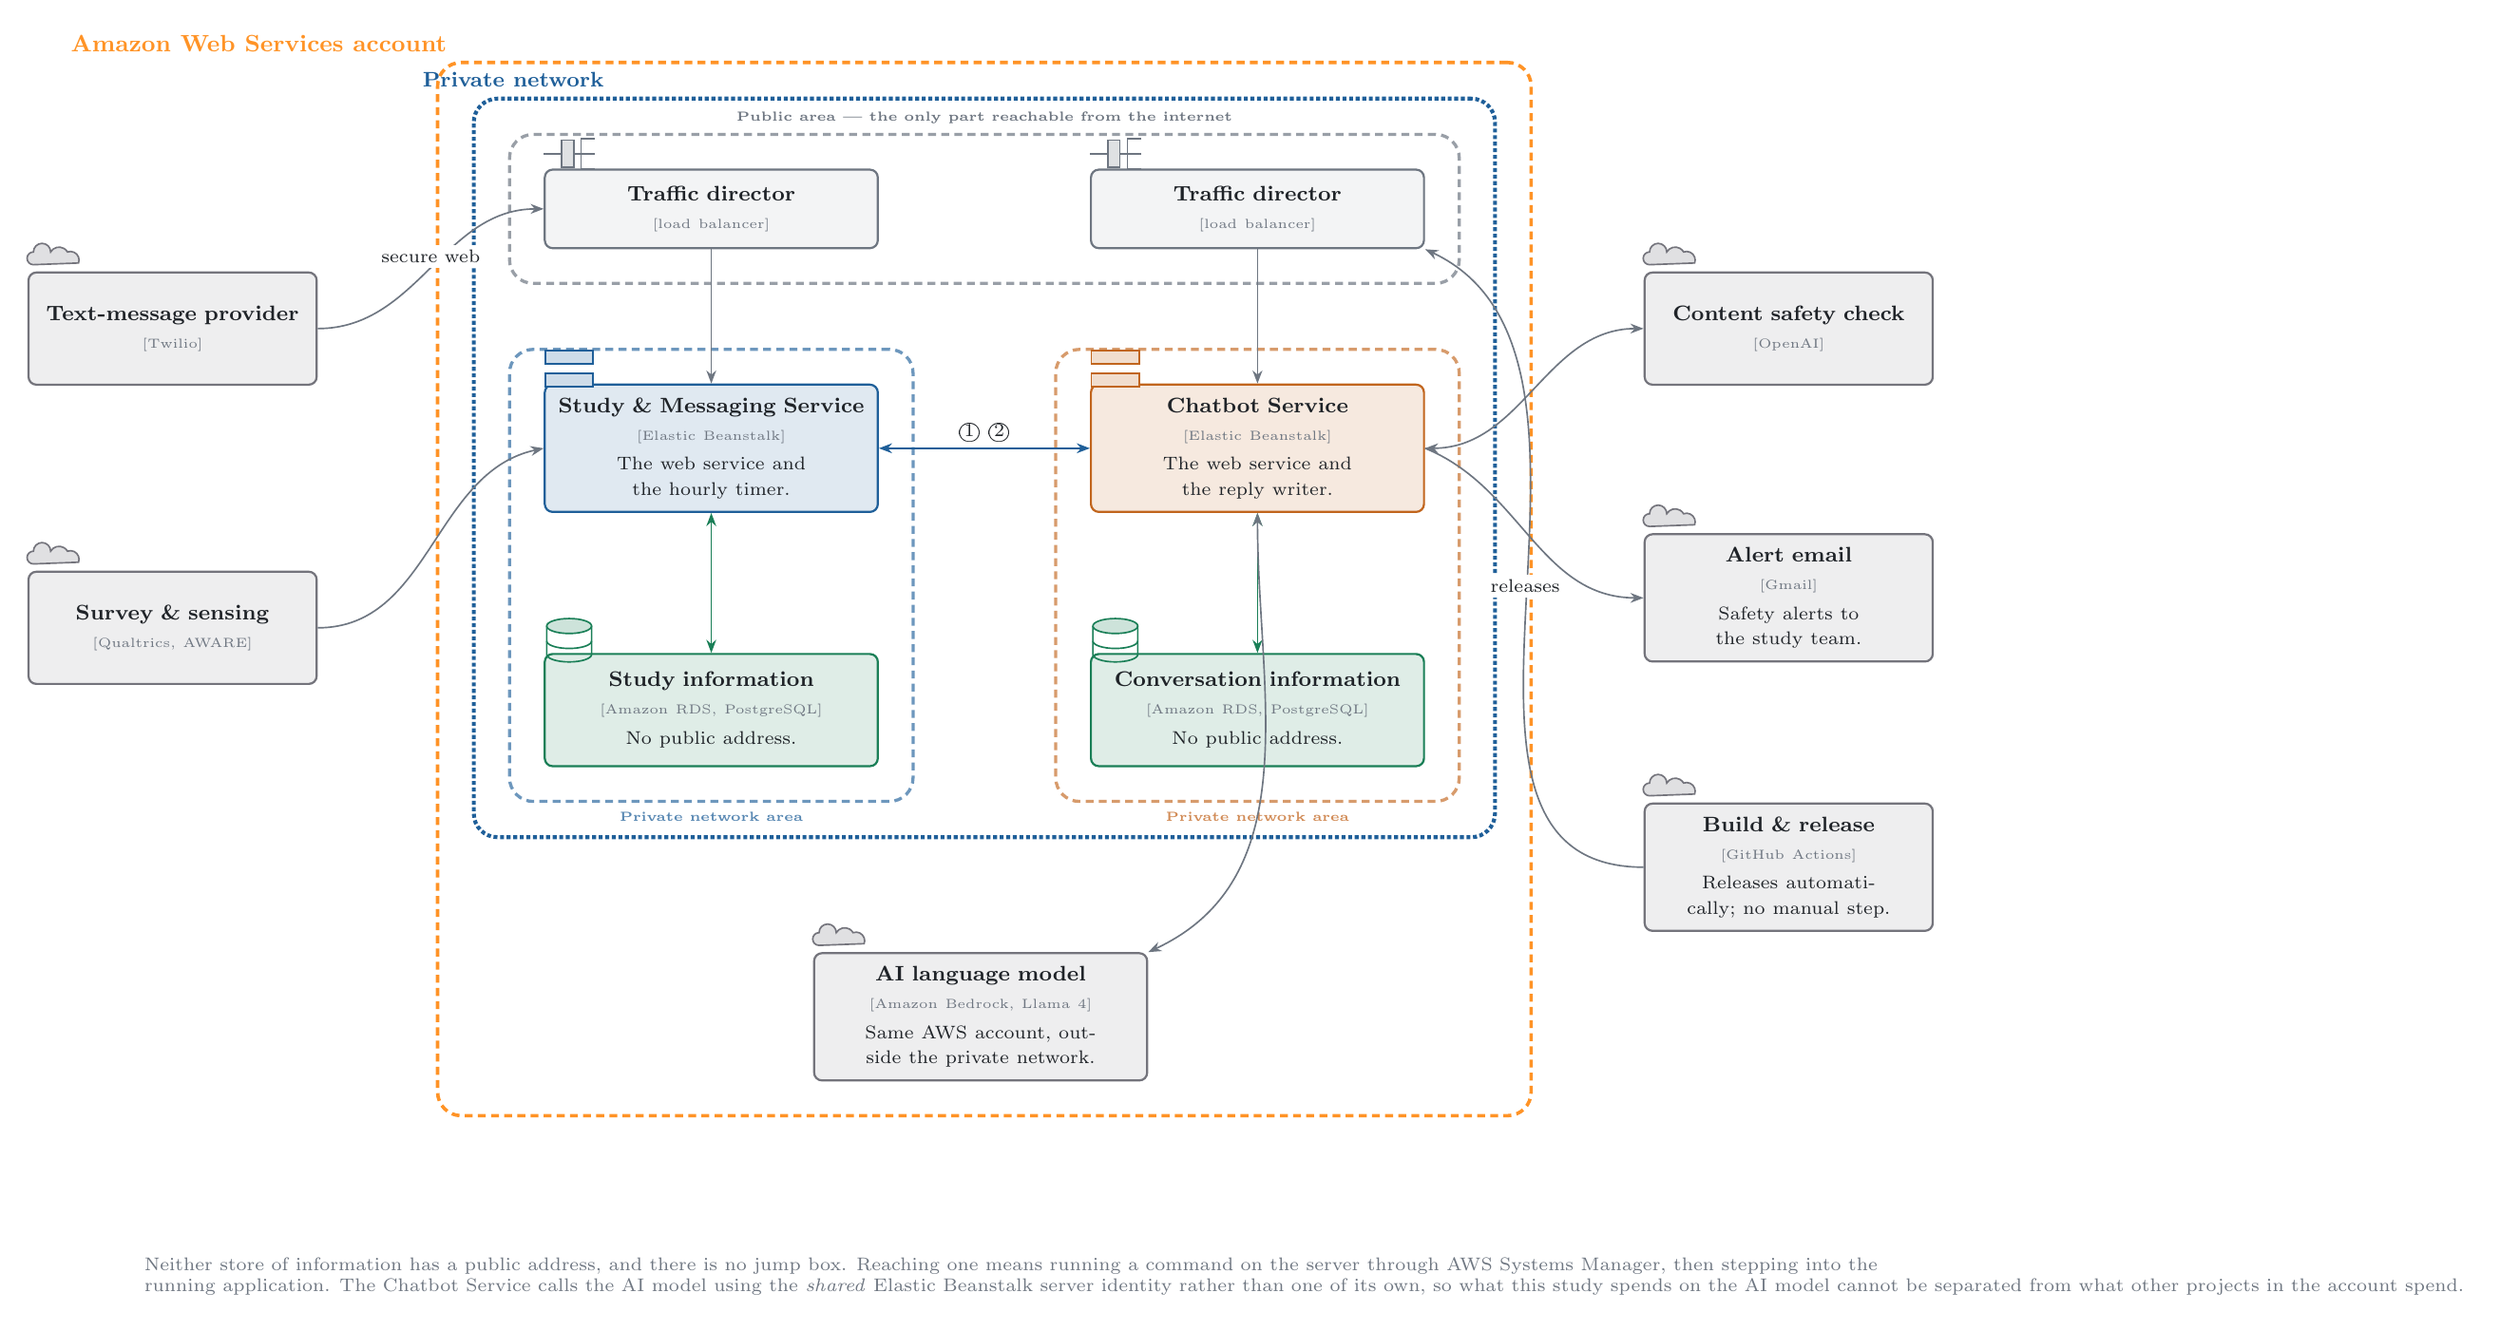
\begin{tikzpicture}

  \node[study, text width=4.1cm] (studyapp) at (5.6,-3.2)
    {\el{Study \& Messaging Service}{Elastic Beanstalk}{The web service and the hourly timer.}};
  \node[store, text width=4.1cm] (studydb) at (5.6,-6.7)
    {\el{Study information}{Amazon RDS, PostgreSQL}{No public address.}};

  \begin{scope}[on background layer]
    \node[bound, draw=studyc!65, fit=(studyapp)(studydb),
          label={[text=studyc!75, font=\tiny\bfseries]below:Private network area}] (studypriv) {};
  \end{scope}

  \node[chat, text width=4.1cm] (chatapp) at (12.9,-3.2)
    {\el{Chatbot Service}{Elastic Beanstalk}{The web service and the reply writer.}};
  \node[store, text width=4.1cm] (chatdb) at (12.9,-6.7)
    {\el{Conversation information}{Amazon RDS, PostgreSQL}{No public address.}};

  \begin{scope}[on background layer]
    \node[bound, draw=chatc!65, fit=(chatapp)(chatdb),
          label={[text=chatc!75, font=\tiny\bfseries]below:Private network area}] (chatpriv) {};
  \end{scope}

  \node[box, fill=mutec!8, draw=mutec, text width=4.1cm, minimum height=1.05cm] (studylb) at (5.6,0)
    {\es{Traffic director}{load balancer}};
  \node[box, fill=mutec!8, draw=mutec, text width=4.1cm, minimum height=1.05cm] (chatlb) at (12.9,0)
    {\es{Traffic director}{load balancer}};

  \begin{scope}[on background layer]
    \node[bound, draw=mutec!70, fit=(studylb)(chatlb),
          label={[text=mutec, font=\tiny\bfseries]above:Public area — the only part reachable from the internet}] (pub) {};
  \end{scope}

  \begin{scope}[on background layer]
    \node[bound, draw=studyc, line width=1.5pt, densely dotted,
          fit=(pub)(studypriv)(chatpriv),
          label={[text=studyc, font=\footnotesize\bfseries]above left:Private network}] (vpc) {};
  \end{scope}

  \node[ext, text width=4.1cm] (ai) at (9.2,-10.8)
    {\el{AI language model}{Amazon Bedrock, Llama 4}{Same AWS account, outside the private network.}};

  \begin{scope}[on background layer]
    \node[bound, draw=orange!85, line width=1.3pt, fit=(vpc)(ai),
          label={[text=orange!85, font=\small\bfseries]above left:Amazon Web Services account}] (aws) {};
  \end{scope}

  \node[ext] (sms) at (-1.6,-1.6) {\el{Text-message provider}{Twilio}{}};
  \node[ext] (survey) at (-1.6,-5.6) {\el{Survey \& sensing}{Qualtrics, AWARE}{}};
  \node[ext] (safety) at (20.0,-1.6) {\el{Content safety check}{OpenAI}{}};
  \node[ext] (mail) at (20.0,-5.2) {\el{Alert email}{Gmail}{Safety alerts to the study team.}};
  \node[ext] (ci) at (20.0,-8.8) {\el{Build \& release}{GitHub Actions}{Releases automatically; no manual step.}};

  \ico{studyapp}{srvicon}{studyc}
  \ico{chatapp}{srvicon}{chatc}
  \ico{studydb}{dbicon}{datac}
  \ico{chatdb}{dbicon}{datac}
  \ico{studylb}{lbicon}{mutec}
  \ico{chatlb}{lbicon}{mutec}
  \ico{ai}{cloudicon}{extc}
  \ico{sms}{cloudicon}{extc}
  \ico{survey}{cloudicon}{extc}
  \ico{safety}{cloudicon}{extc}
  \ico{mail}{cloudicon}{extc}
  \ico{ci}{cloudicon}{extc}

  \draw[arr] (sms.east) to[out=0, in=180] node[lbl, above]{secure web} (studylb.west);
  \draw[arr] (survey.east) to[out=0, in=192] (studyapp.west);
  \draw[arr] (studylb) -- (studyapp);
  \draw[arr] (chatlb) -- (chatapp);
  \draw[darr, draw=datac] (studyapp) -- (studydb);
  \draw[darr, draw=datac] (chatapp) -- (chatdb);
  \draw[darr, draw=studyc, thick] (studyapp.east) --
    node[lbl, above]{\textcircled{1} \textcircled{2}} (chatapp.west);
  \draw[darr] (chatapp.south) to[out=-90, in=25] (ai.north east);
  \draw[darr] (chatapp.east) to[out=0, in=180] (safety.west);
  \draw[arr] (chatapp.east) to[out=-22, in=180] (mail.west);
  \draw[arr] (ci.west) to[out=180, in=-25] node[lbl, above]{releases} (chatlb.south east);

  \node[note, anchor=north west] at (-2.1,-13.9)
    {Neither store of information has a public address, and there is no jump box. Reaching one means
     running a command on the server through AWS Systems Manager, then stepping into the\\
     running application. The Chatbot Service calls the AI model using the \emph{shared} Elastic
     Beanstalk server identity rather than one of its own, so what this study spends on the AI model
     cannot be separated from what other projects in the account spend.};

\end{tikzpicture}

\vspace{10pt}
\legend
\end{center}
\vfill

\clearpage

%% ════════════════════════════════════════════════
%% 4 — MESSAGE JOURNEY
%% A sequence view in plain sentences. Every step is
%% something happening, not a function being called.
%% ════════════════════════════════════════════════
\null\vfill
\begin{center}
\pagehead{4 — What happens to one message}{%
  A participant sends a text and gets a reply. Read top to bottom; each numbered step
  is one thing happening.}{%
  SMART-R text-messaging study \textbullet\ August 2026 \textbullet\
  Scope: one incoming message. A daily opener is simply filed and skips steps 6--11.}

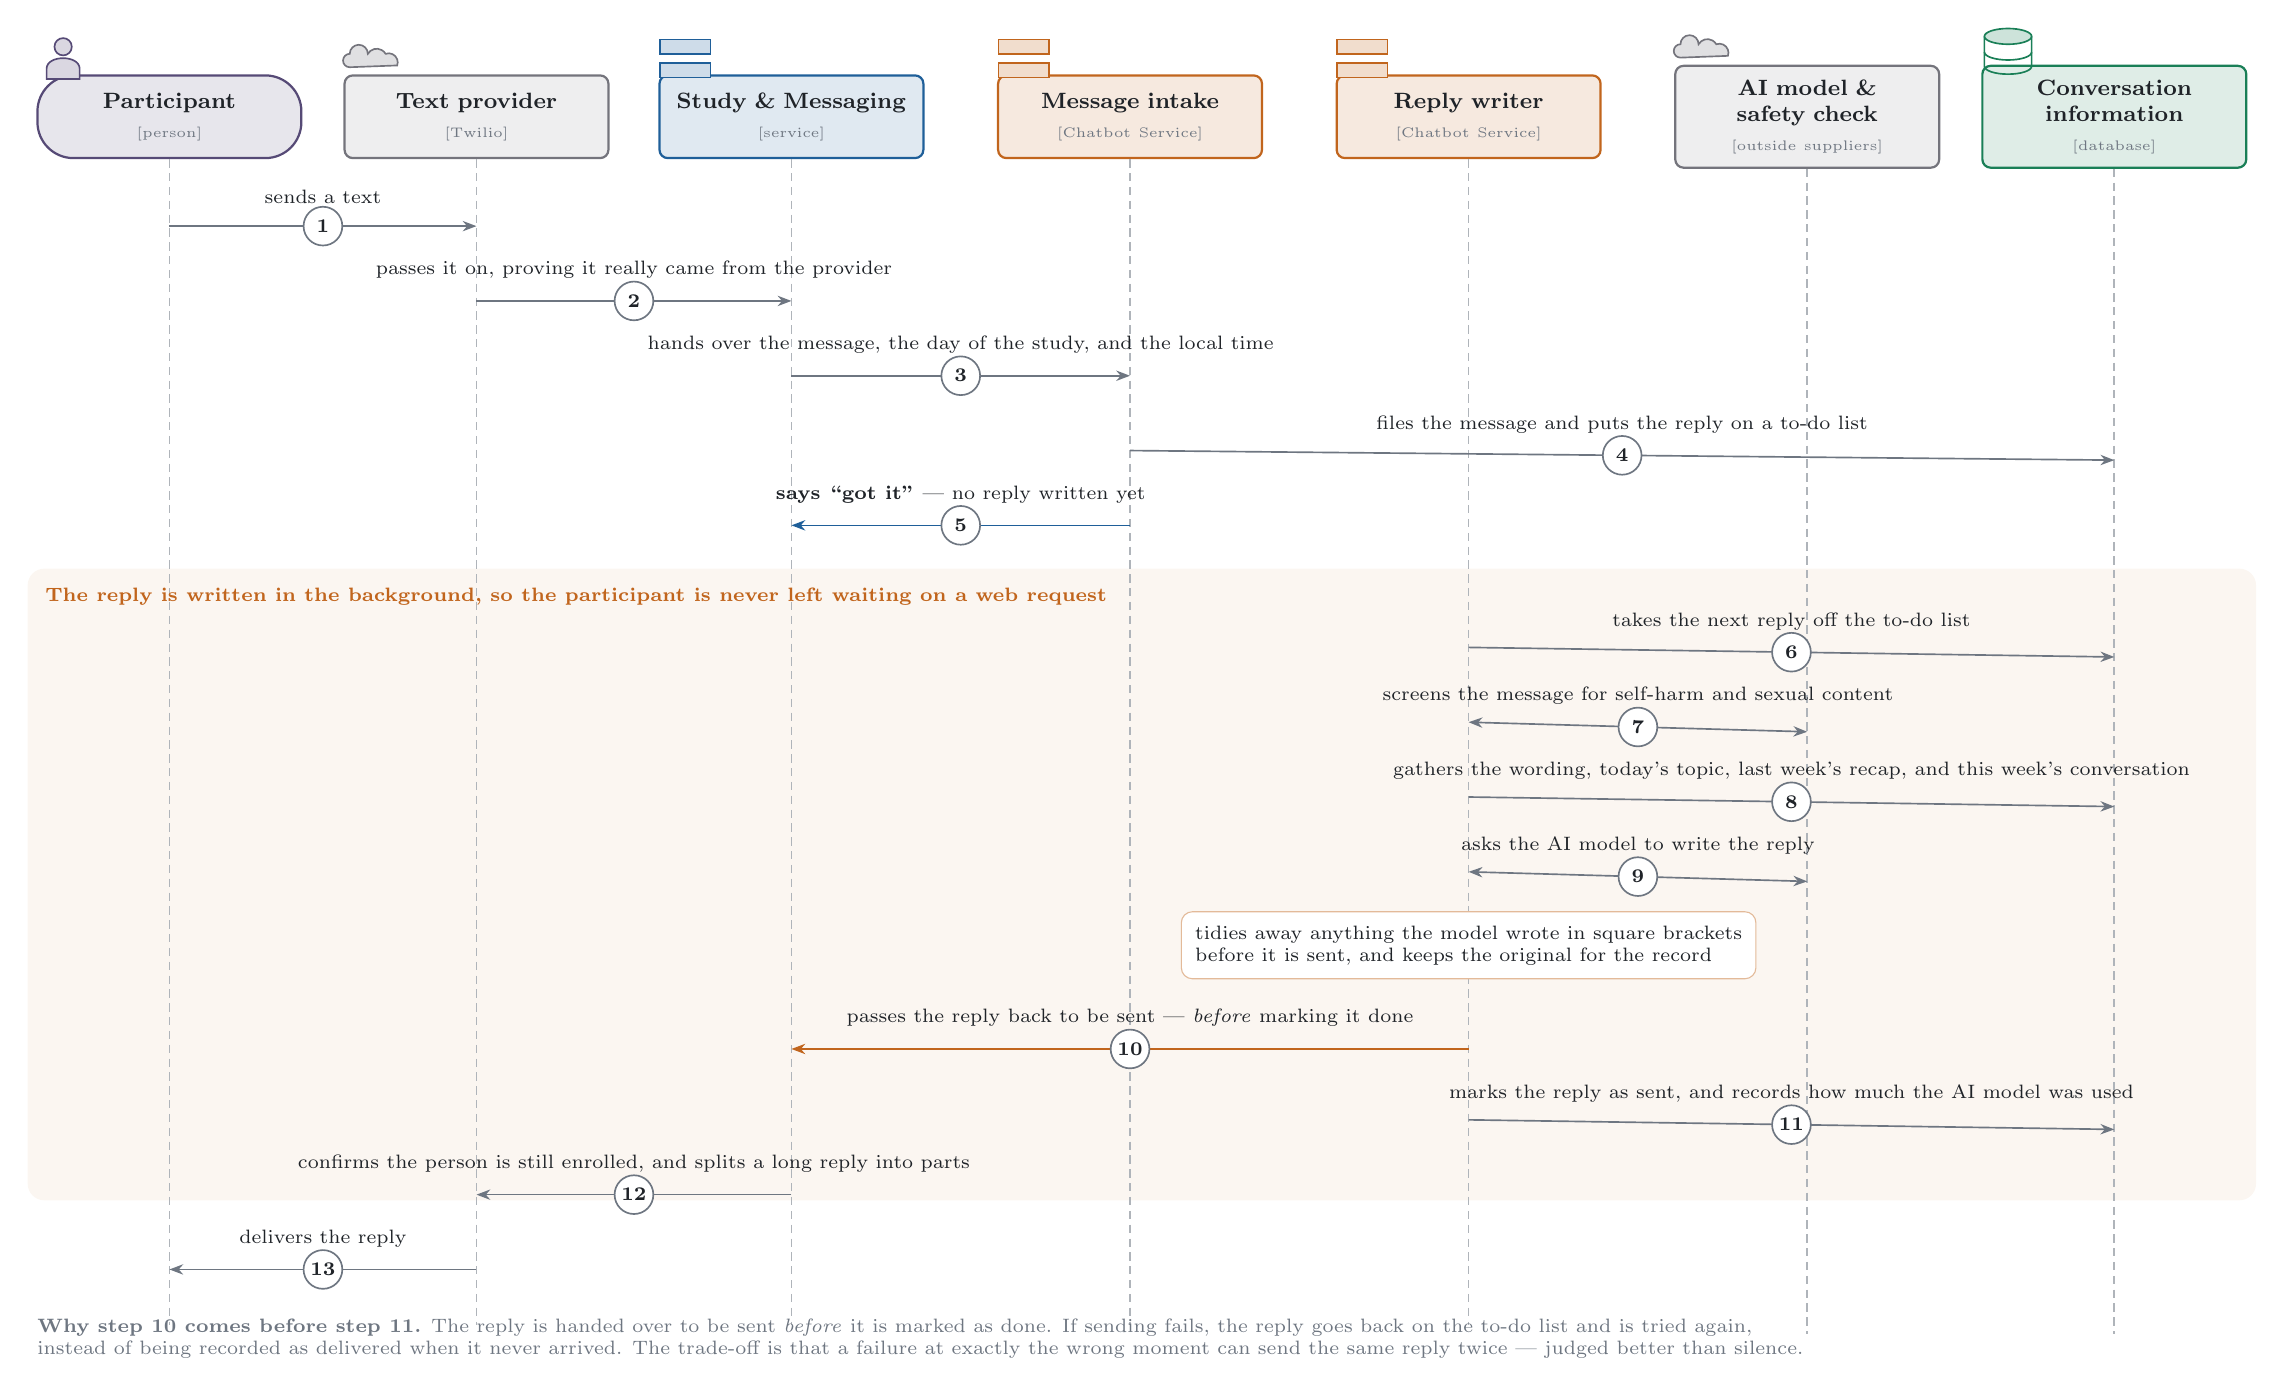
\begin{tikzpicture}

  \def\ybot{-14.8}

  \node[person, text width=3.0cm, minimum height=1.05cm] (a1) at (0,0)
    {\es{Participant}{person}};
  \node[ext, text width=3.0cm, minimum height=1.05cm] (a2) at (3.9,0)
    {\es{Text provider}{Twilio}};
  \node[study, text width=3.0cm, minimum height=1.05cm] (a3) at (7.9,0)
    {\es{Study \& Messaging}{service}};
  \node[chat, text width=3.0cm, minimum height=1.05cm] (a4) at (12.2,0)
    {\es{Message intake}{Chatbot Service}};
  \node[chat, text width=3.0cm, minimum height=1.05cm] (a5) at (16.5,0)
    {\es{Reply writer}{Chatbot Service}};
  \node[ext, text width=3.0cm, minimum height=1.05cm] (a6) at (20.8,0)
    {\es{AI model \& safety check}{outside suppliers}};
  \node[store, text width=3.0cm, minimum height=1.05cm] (a7) at (24.7,0)
    {\es{Conversation information}{database}};

  \foreach \n in {a1,a2,a3,a4,a5,a6,a7} {
    \draw[life] (\n.south) -- ($(\n.south) + (0,\ybot)$);
  }

  \ico{a1}{personicon}{personc}
  \ico{a2}{cloudicon}{extc}
  \ico{a3}{srvicon}{studyc}
  \ico{a4}{srvicon}{chatc}
  \ico{a5}{srvicon}{chatc}
  \ico{a6}{cloudicon}{extc}
  \ico{a7}{dbicon}{datac}

  \newcommand{\hop}[5]{%
    \draw[arr] ($(#1.south) + (0,#3)$) -- ($(#2.south) + (0,#3)$) node[num, pos=0.5]{#4};
    \node[font=\scriptsize, text=inkc, anchor=south, align=center]
      at ($($(#1.south)!0.5!(#2.south)$) + (0,#3+0.16)$) {#5};}
  \newcommand{\hopb}[5]{%
    \draw[darr] ($(#1.south) + (0,#3)$) -- ($(#2.south) + (0,#3)$) node[num, pos=0.5]{#4};
    \node[font=\scriptsize, text=inkc, anchor=south, align=center]
      at ($($(#1.south)!0.5!(#2.south)$) + (0,#3+0.16)$) {#5};}

  \hop{a1}{a2}{-0.85}{1}{sends a text}
  \hop{a2}{a3}{-1.8}{2}{passes it on, proving it really came from the provider}
  \hop{a3}{a4}{-2.75}{3}{hands over the message, the day of the study, and the local time}
  \hop{a4}{a7}{-3.7}{4}{files the message and puts the reply on a to-do list}

  \draw[arr, draw=studyc] ($(a4.south) + (0,-4.65)$) -- ($(a3.south) + (0,-4.65)$)
    node[num, pos=0.5]{5};
  \node[font=\scriptsize, text=inkc, anchor=south]
    at ($($(a3.south)!0.5!(a4.south)$) + (0,-4.49)$)
    {\textbf{says ``got it''} — no reply written yet};

  \begin{scope}[on background layer]
    \fill[chatc!6, rounded corners=6pt]
      ($(a1.south) + (-1.8,-5.2)$) rectangle ($(a7.south) + (1.8,-13.1)$);
  \end{scope}
  \node[font=\scriptsize\bfseries, text=chatc, anchor=west]
    at ($(a1.south) + (-1.7,-5.55)$)
    {The reply is written in the background, so the participant is never left waiting on a web request};

  \hop{a5}{a7}{-6.2}{6}{takes the next reply off the to-do list}
  \hopb{a5}{a6}{-7.15}{7}{screens the message for self-harm and sexual content}
  \hop{a5}{a7}{-8.1}{8}{gathers the wording, today's topic, last week's recap, and this week's conversation}
  \hopb{a5}{a6}{-9.05}{9}{asks the AI model to write the reply}

  \node[draw=chatc!45, fill=white, rounded corners=4pt, inner sep=5pt,
        font=\scriptsize, align=left, text=inkc, anchor=north]
    at ($(a5.south) + (0,-9.55)$)
    {tidies away anything the model wrote in square brackets\\
     before it is sent, and keeps the original for the record};

  \draw[arr, draw=chatc] ($(a5.south) + (0,-11.3)$) -- ($(a3.south) + (0,-11.3)$)
    node[num, pos=0.5]{10};
  \node[font=\scriptsize, text=inkc, anchor=south]
    at ($($(a3.south)!0.5!(a5.south)$) + (0,-11.14)$)
    {passes the reply back to be sent — \emph{before} marking it done};

  \hop{a5}{a7}{-12.2}{11}{marks the reply as sent, and records how much the AI model was used}
  \hop{a3}{a2}{-13.15}{12}{confirms the person is still enrolled, and splits a long reply into parts}
  \hop{a2}{a1}{-14.1}{13}{delivers the reply}

  \node[note, anchor=north west] at ($(a1.south) + (-1.8,-14.6)$)
    {\textbf{Why step 10 comes before step 11.} The reply is handed over to be sent \emph{before} it is
     marked as done. If sending fails, the reply goes back on the to-do list and is tried again,\\
     instead of being recorded as delivered when it never arrived. The trade-off is that a failure at
     exactly the wrong moment can send the same reply twice — judged better than silence.};

\end{tikzpicture}

\vspace{10pt}
\legend
\end{center}
\vfill

\end{document}
